\section{Resultados preliminares}
\label{sec:resultados}

\textbf{Metodología de medición.} El programa \texttt{Benchmark} mide el
tiempo por operación para $n \in \{10^3, 10^4, 10^5, 10^6\}$ solicitudes
pendientes, con urgencias uniformes entre 1 y 5 generadas con semilla fija.
Cada medición se ejecuta dos veces como calentamiento del compilador JIT y
cinco veces más, y se reporta la mediana. Se usó OpenJDK~21 en un
contenedor Linux con dos núcleos (Intel Xeon a 2{,}1~GHz) y \texttt{-Xmx2g}.
Los datos completos están en \texttt{results/benchmark.csv}. Son
resultados preliminares de un solo equipo, por lo que deben leerse como
tendencias y no como valores absolutos.

\textbf{Operaciones del sistema.} La Tabla~\ref{tab:sistema} muestra que
todas las operaciones principales cuestan del orden de $10^2$~ns sin
importar $n$: al multiplicar $n$ por mil, el tiempo varía a lo sumo en un
factor de 4, mientras que una operación lineal habría crecido mil veces.
Ese aumento moderado para $n=10^6$ se explica por la jerarquía de memoria:
con un millón de nodos, los datos ya no caben en la caché del procesador y
cada acceso al índice o a un nodo es más lento, aunque el número de pasos
no cambie. El valor alto de registrar con $n=10^3$ se debe a que esa
medición incluye los primeros redimensionamientos de la tabla y código aún
no optimizado por el JIT.

\begin{table}[t]
  \caption{Tiempo por operación de \texttt{TriageSystem} (ns, mediana)}
  \label{tab:sistema}
  \centering
  \footnotesize
  \begin{tabular}{rrrrrr}
    \toprule
    $n$ & Registrar & Buscar & Cancelar & Atender & Deshacer \\
    \midrule
    $10^3$ & 912 & 62 & 272 & 97 & 91 \\
    $10^4$ & 137 & 97 & 152 & 106 & 118 \\
    $10^5$ & 268 & 85 & 159 & 59 & 114 \\
    $10^6$ & 307 & 233 & 428 & 141 & 139 \\
    \bottomrule
  \end{tabular}
\end{table}

\textbf{Índice hash frente a búsqueda lineal.} La
Fig.~\ref{fig:busqueda} compara la búsqueda de la Entrega 1 con la actual
(1\,000 búsquedas de identificadores existentes al azar). La búsqueda lineal
crece aproximadamente en proporción a $n$ (algo más entre $10^4$ y $10^5$,
cuando las listas dejan de caber en la caché) y llega a 12~ms por consulta con $10^6$
pendientes; con el índice, la consulta tarda 0{,}19~$\mu$s, unas 63\,000
veces menos. El mismo efecto aparece al registrar: verificar duplicados
recorriendo las colas hace que registrar $3\times10^4$ solicitudes cueste
275~$\mu$s por registro, frente a 0{,}1~$\mu$s con el índice; el costo total
de la Entrega 1 era $\Theta(n^2)$.

\begin{figure}[t]
  \centering
  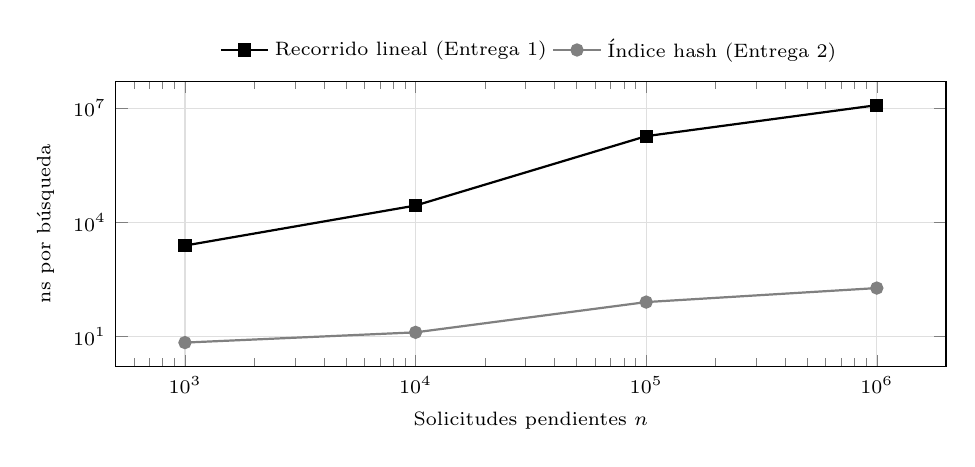
\begin{tikzpicture}
    \begin{loglogaxis}[
        width=\columnwidth, height=5.2cm,
        xlabel={Solicitudes pendientes $n$},
        ylabel={ns por búsqueda},
        legend style={font=\scriptsize, at={(0.5,1.03)}, anchor=south,
          legend columns=2, draw=none},
        tick label style={font=\scriptsize}, label style={font=\scriptsize},
        grid=major, grid style={gray!25}]
      \addplot[mark=square*, thick] coordinates
        {(1000,2467) (10000,27770) (100000,1840793) (1000000,11991043)};
      \addlegendentry{Recorrido lineal (Entrega 1)}
      \addplot[mark=*, thick, gray] coordinates
        {(1000,7) (10000,13) (100000,81) (1000000,189)};
      \addlegendentry{Índice hash (Entrega 2)}
    \end{loglogaxis}
  \end{tikzpicture}
  \caption{Tiempo de búsqueda por identificador (escala logarítmica en
  ambos ejes).}
  \label{fig:busqueda}
\end{figure}

\textbf{Alternativas de cola de prioridad.} La Fig.~\ref{fig:colas} mide
insertar $n$ solicitudes y luego extraerlas todas, comparando la cola por
niveles con un \emph{heap} binario (\texttt{java.util.PriorityQueue} con
comparador por urgencia y llegada) y con una lista enlazada ordenada,
implementada solo para esta comparación. La cola por niveles es entre 6 y 9
veces más rápida que el \emph{heap}, cuyo costo crece con $\log n$, y la
lista ordenada empeora linealmente por operación (52~$\mu$s con
$n=3\times10^4$); por eso no se midió con tamaños mayores. El resultado
confirma la decisión de diseño de la Sección~\ref{sec:metodologia}: con
pocos niveles fijos, las cubetas superan a la estructura de propósito
general.

\begin{figure}[t]
  \centering
  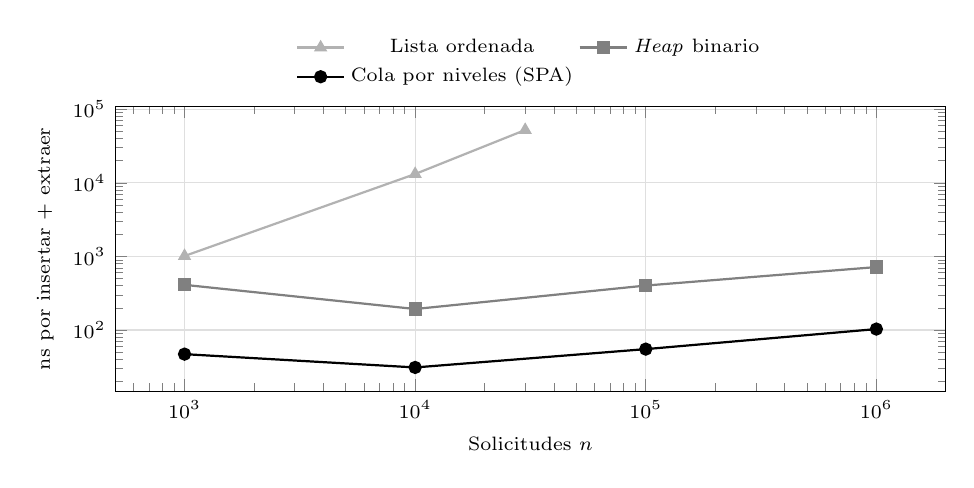
\begin{tikzpicture}
    \begin{loglogaxis}[
        width=\columnwidth, height=5.2cm,
        xlabel={Solicitudes $n$},
        ylabel={ns por insertar + extraer},
        legend style={font=\scriptsize, at={(0.5,1.03)}, anchor=south,
          legend columns=2, draw=none},
        tick label style={font=\scriptsize}, label style={font=\scriptsize},
        grid=major, grid style={gray!25}]
      \addplot[mark=triangle*, thick, gray!60] coordinates
        {(1000,1013) (10000,13178) (30000,52238)};
      \addlegendentry{Lista ordenada}
      \addplot[mark=square*, thick, gray] coordinates
        {(1000,411) (10000,193) (100000,402) (1000000,717)};
      \addlegendentry{\emph{Heap} binario}
      \addplot[mark=*, thick] coordinates
        {(1000,47) (10000,31) (100000,55) (1000000,103)};
      \addlegendentry{Cola por niveles (SPA)}
    \end{loglogaxis}
  \end{tikzpicture}
  \caption{Costo de las tres representaciones de la cola de prioridad.}
  \label{fig:colas}
\end{figure}

\textbf{Memoria.} Con $10^6$ pendientes, el sistema ocupa unos 97 bytes por
solicitud (medido con la memoria usada por la JVM antes y después de
registrar, sin contar las cadenas de los identificadores). Ese espacio se
reparte entre el \texttt{Ticket}, el nodo de la lista doble, la entrada de
la tabla hash y su parte del arreglo de cubetas; es el precio, lineal en
$n$, de las operaciones en tiempo constante.
